\section{Actividad 1: Corriente de Saturación $I_{DSS}$}

\subsection{Simulación}

Para la primera simulacion vamos a implementar el siguiente circuito al simulador (LTSpice).

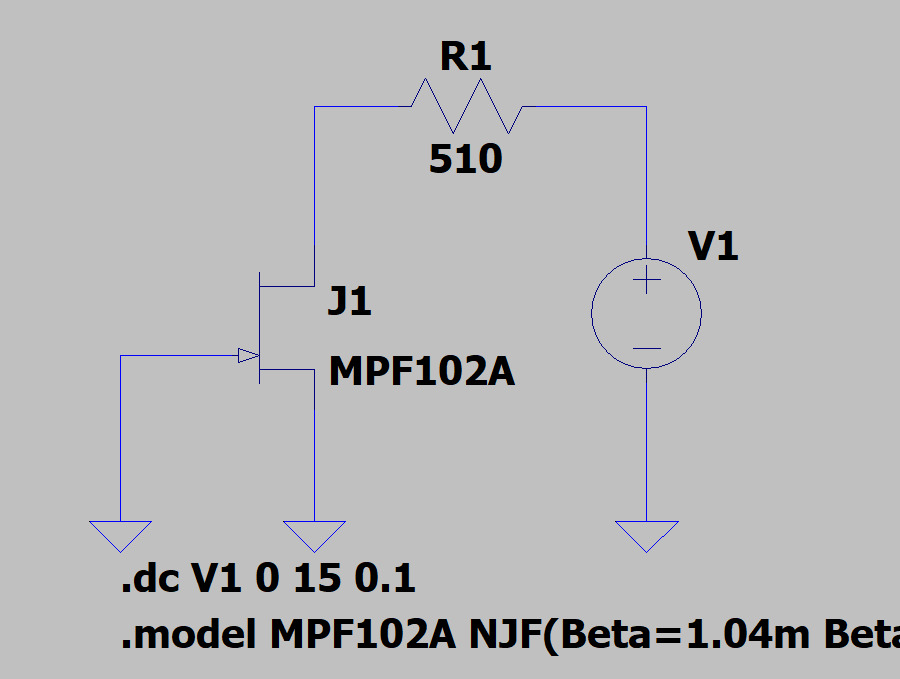
\includegraphics[width=6cm]{./imagenes/Circ1.png}

Observando el comportamiento de $I_DS$ con respecto a $V_{DS}$, obtenemos la siguiente gráfica:


Podemos ver que el valor de $I_{DSS}$ es PONER VALOR, lo cual difiere con el obtenido en la hoja de datos el cual es de 20mA

\subsection{Laboratorio}

\paragraph{Instrumental y Materiales}
\begin{itemize}
    \item Multimetro UNI-T UT89X
    \item Transistor JFET MPF102
    \item Resistor de
    \item Fuente de alimentación
\end{itemize}

\paragraph{Procedimiento}